% Standalone, editable timeline of one example patient under three policies.
%   pdflatex fig_timeline_standalone.tex
% Example: onset at 0, pickup at 60 min; nearest hospital is a non-stroke-center 8 min
% away, nearest thrombolysis-capable center 12 min, nearest EVT-capable center 25 min;
% transfer leg to the EVT center 25 min; base-case intervals DTN 45, DTP 90 / 60 (transfer),
% DIDO 121. Edit the numbers in the \timeline calls below.
\documentclass[tikz, border=4pt]{standalone}
\usepackage[T1]{fontenc}
\usepackage{mathptmx}  % Times text and math, matching the IEEEtran body
\usepackage{amsmath}
\usetikzlibrary{arrows.meta, calc}

\begin{document}
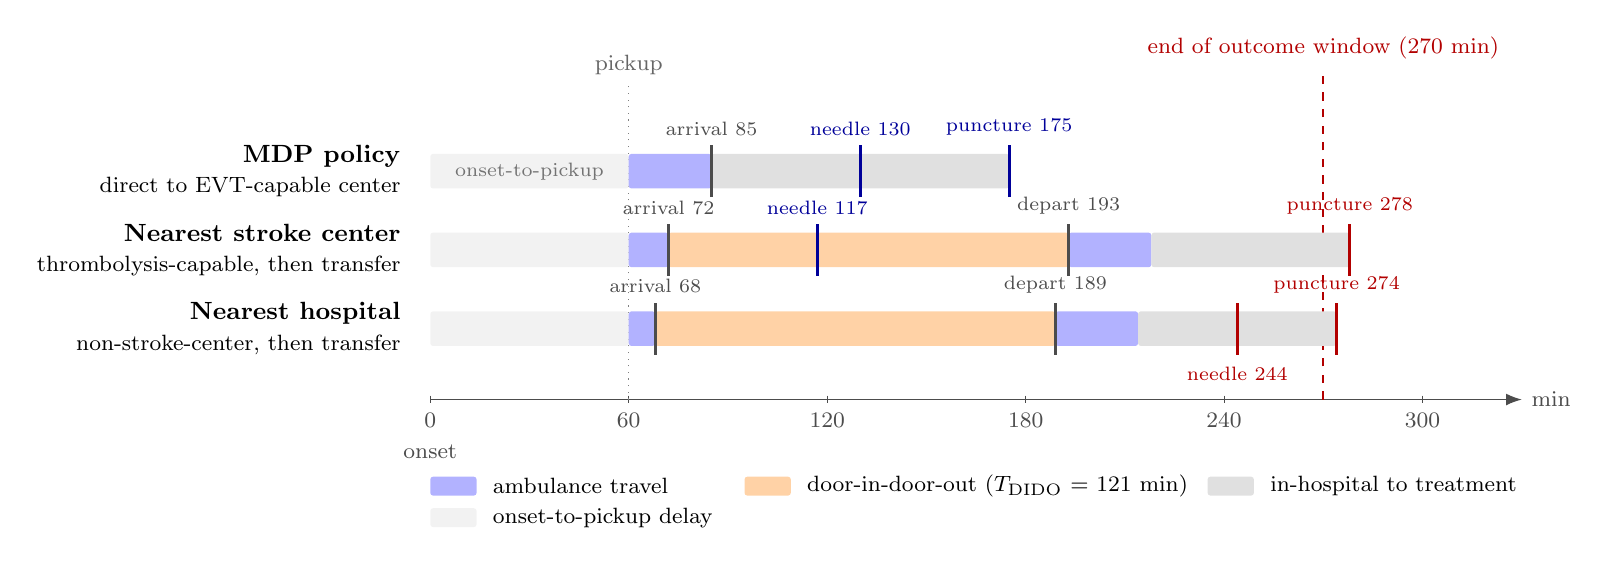
\begin{tikzpicture}[x=0.042cm, y=1cm, font=\small]
\def\ymax{3}
% ---- time axis
\draw[-{Latex[length=2mm]}, black!70] (0,-0.9) -- (330,-0.9) node[right, font=\footnotesize] {min};
\foreach \t in {0,60,...,300} {\draw[black!70] (\t,-0.85) -- (\t,-0.95) node[below, font=\footnotesize] {\t};}
\node[font=\footnotesize, black!70, anchor=north] at (0,-1.35) {onset};
% ---- outcome window
\draw[red!70!black, dashed, line width=0.7pt] (270,-0.9) -- (270,\ymax+0.3);
\node[font=\footnotesize, red!70!black, anchor=south] at (270,\ymax+0.3) {end of outcome window (270 min)};
% ---- pickup marker
\draw[black!50, dotted] (60,-0.9) -- (60,\ymax+0.1);
\node[font=\footnotesize, black!60, anchor=south] at (60,\ymax+0.1) {pickup};

% segment styles
\tikzset{travel/.style={fill=blue!30, draw=none},
         wait/.style={fill=black!12, draw=none},
         dido/.style={fill=orange!35, draw=none},
         bar/.style={rounded corners=1pt}}
\def\h{0.22}
% \seg{y}{from}{to}{style}
\newcommand{\seg}[4]{\fill[#4, bar] (#2,#1-\h) rectangle (#3,#1+\h);}
% \tick{y}{t}{label}{color}
\newcommand{\tick}[4]{\draw[#4, line width=1pt] (#2,#1-0.33) -- (#2,#1+0.33); \node[font=\scriptsize, #4, anchor=south] at (#2,#1+0.33) {#3};}

% pre-pickup delay (onset to departure), same for all policies
\foreach \yy in {0,1,2} {\fill[black!5, bar] (0,\yy-\h) rectangle (60,\yy+\h);}
\node[font=\scriptsize, black!55] at (30,2) {onset-to-pickup};

% ===== lane 1: MDP / nearest EVT-capable center (direct) at y = 2
\node[anchor=east, align=right, font=\small] at (-6,2) {\textbf{MDP policy}\\\footnotesize direct to EVT-capable center};
\seg{2}{60}{85}{travel}            % 25 min drive
\seg{2}{85}{175}{wait}             % in-hospital to puncture
\tick{2}{85}{arrival 85}{black!70}
\tick{2}{130}{needle 130}{blue!60!black}
\tick{2}{175}{puncture 175}{blue!60!black}

% ===== lane 2: nearest stroke center (thrombolysis-capable, then transfer) at y = 1
\node[anchor=east, align=right, font=\small] at (-6,1) {\textbf{Nearest stroke center}\\\footnotesize thrombolysis-capable, then transfer};
\seg{1}{60}{72}{travel}            % 12 min drive
\seg{1}{72}{193}{dido}             % DIDO 121
\seg{1}{193}{218}{travel}          % transfer 25 min
\seg{1}{218}{278}{wait}            % DTP transfer 60
\tick{1}{72}{arrival 72}{black!70}
\tick{1}{117}{needle 117}{blue!60!black}
\tick{1}{193}{depart 193}{black!70}
\tick{1}{278}{puncture 278}{red!70!black}

% ===== lane 3: nearest hospital (non-stroke-center, then transfer) at y = 0
\node[anchor=east, align=right, font=\small] at (-6,0) {\textbf{Nearest hospital}\\\footnotesize non-stroke-center, then transfer};
\seg{0}{60}{68}{travel}            % 8 min drive
\seg{0}{68}{189}{dido}             % DIDO 121
\seg{0}{189}{214}{travel}          % transfer 25 min
\seg{0}{214}{274}{wait}            % DTP transfer 60
\tick{0}{68}{arrival 68}{black!70}
\tick{0}{189}{depart 189}{black!70}
\draw[red!70!black, line width=1pt] (244,-0.33) -- (244,0.33); \node[font=\scriptsize, red!70!black, anchor=north] at (244,-0.36) {needle 244};
\tick{0}{274}{puncture 274}{red!70!black}

% ---- legend
\begin{scope}[shift={(0,-2.0)}]
  \fill[travel, bar] (0,-0.12) rectangle (14,0.12); \node[anchor=west, font=\footnotesize] at (16,0) {ambulance travel};
  \fill[dido, bar] (95,-0.12) rectangle (109,0.12); \node[anchor=west, font=\footnotesize] at (111,0) {door-in-door-out ($T_{\mathrm{DIDO}}$ = 121 min)};
  \fill[wait, bar] (235,-0.12) rectangle (249,0.12); \node[anchor=west, font=\footnotesize] at (251,0) {in-hospital to treatment};
  \fill[black!5, bar] (0,-0.52) rectangle (14,-0.28); \node[anchor=west, font=\footnotesize] at (16,-0.4) {onset-to-pickup delay};
\end{scope}
\end{tikzpicture}
\end{document}
